\documentclass[11pt,a4paper]{article}

\usepackage[margin=2.5cm]{geometry}
\usepackage{amsmath,amssymb}
\usepackage{graphicx}
\usepackage{booktabs}
\usepackage[round,authoryear]{natbib}
\usepackage{xcolor}
\usepackage[colorlinks=true,linkcolor=blue!50!black,citecolor=blue!50!black,urlcolor=blue!50!black]{hyperref}

\graphicspath{{../../figures/}}

\newcommand{\cl}{\mathrm{cl}}
\newcommand{\dchi}{\Delta\chi^2}

\title{CMB constraints on compact baryonic clumps as part of the dark matter:\\ summary for discussion}
\author{S\textperiodcentered HARDY\textperiodcentered HOC\textperiodcentered PER\textperiodcentered CLAVDIVM\textperiodcentered FIERI\textperiodcentered IVSSIT}
\date{14 October 2026}

\begin{document}
\maketitle

\section{Purpose}

This note summarises what the Planck CMB data say about compact, pressureless clumps of baryonic matter that make up some or all of the dark matter, and where clouds of the kind proposed by \citet{WalkerWardle1998} fall in that picture. The background physics is set out in the explainer (\texttt{doc/explainer/clumps\_explainer.pdf}) and the analysis for clumps that make up all of the dark matter in the report (\texttt{doc/report/cmb\_bound\_report.pdf}). This note adds the case in which only a fraction of the dark matter is in clumps.

\section{The question and the model}

The question is conditional: if clumps exist throughout the epochs that matter for the CMB, how strongly can they be coupled to the radiation? Formation, survival and Big Bang nucleosynthesis (BBN) are separate questions about whether such clumps can exist, and are discussed in Section~\ref{sec:caveats}.

The clumps exchange momentum with the photons through a momentum-transfer cross-section $\sigma$. The CMB is sensitive only to the cross-section per unit mass, expressed in \textsc{class} by the dimensionless coupling
\begin{equation}
u = \frac{\sigma}{\sigma_T}\left(\frac{M}{100\,\mathrm{GeV}}\right)^{-1},
\qquad \frac{\sigma}{M} = \frac{u}{268}\,\mathrm{cm^2\,g^{-1}} .
\end{equation}
For an optically thick clump $\sigma = Q\,\pi R^2$ with $Q$ of order unity ($Q=1$ for an absorber), so a limit on $u$ is a limit on the surface density,
\begin{equation}
\frac{\Sigma}{Q} = \frac{M}{Q\,\pi R^2} = \frac{268}{u}\,\mathrm{g\,cm^{-2}} .
\end{equation}
The CMB signal comes from radiation drag on the clumps before recombination, which suppresses the growth of their density perturbations. Planck sees this mainly through reduced gravitational lensing of the CMB. Photons scattering off the clumps is a negligible effect at $f_\cl = 1$ but becomes important at small $f_\cl$ and strong coupling (Section~\ref{sec:results}).

For the mixture, a fraction $f_\cl$ of the dark matter is in clumps and the rest is collisionless cold dark matter (CDM):
\begin{equation}
\omega_\cl = f_\cl\,\omega_{\rm dark}, \qquad \omega_{\rm CDM} = (1-f_\cl)\,\omega_{\rm dark}.
\end{equation}
The total $\omega_{\rm dark}$, the diffuse baryon density $\omega_b$, the other four $\Lambda$CDM parameters and the nine likelihood nuisance parameters are all fitted. Two angular laws for the photon--clump interaction are compared at equal $u$: Thomson scattering, which generates polarization, and uniform re-emission in the clump frame with no polarization, which is the appropriate limit for an opaque body.

\section{Data and method}

The likelihood is the Planck PR4 CamSpec high-$\ell$ TT, TE and EE likelihood with the Planck 2018 low-$\ell$ TT and EE likelihoods. The spectra are computed with \textsc{class}~3.4.0, patched to allow the second kernel, and with tighter numerical settings than the defaults. For each fixed $(f_\cl, u)$ the objective is minimised over the other fifteen parameters (a profile likelihood). Results are given as
\begin{itemize}
\item $\dchi$ relative to the best $\Lambda$CDM fit, and
\item nominal fixed-fraction thresholds: the coupling at which $\dchi$ rises 2.71 above that fraction's own minimum. These are not joint confidence regions in $(f_\cl, u)$.
\end{itemize}
About 150 profile points were computed. Repeated fits agree to about 0.02 in $\dchi$. Changing the tight-coupling approximation or the numerical precision changes $\chi^2$ by at most about 0.1 relative to $\Lambda$CDM at every point checked, including the strongest couplings.

\section{Results}
\label{sec:results}

\subsection{All of the dark matter in clumps}

From the report: $u < 1.1\times10^{-4}$ (profile, PR4 CamSpec; $1.0\times10^{-4}$ with Planck 2018 plik), and $u < 1.7\times10^{-4}$ from a Bayesian analysis with a flat prior on $u$. These correspond to $\Sigma/Q \gtrsim 2\times10^{6}\,\mathrm{g\,cm^{-2}}$, about the column density of ten kilometres of rock. The kernel changes this by about 3\%.

\subsection{A fraction of the dark matter in clumps}

\begin{table}[t]
\centering
\small
\caption{Nominal fixed-fraction thresholds ($\dchi = 2.71$ above each fraction's own profile minimum), PR4 CamSpec with 2018 low-$\ell$. ``Not reached'' means no threshold within the computed range, whose smallest $\Sigma/Q$ is given in brackets. The last column is the depth of the profile minimum relative to $\Lambda$CDM for the isotropic kernel.}
\label{tab:thresholds}
\begin{tabular}{lcccc}
\toprule
$f_\cl$ & $\Sigma/Q$ [g\,cm$^{-2}$], Thomson & $\Sigma/Q$ [g\,cm$^{-2}$], isotropic & $u$ (Thomson) & min.\ $-$ $\Lambda$CDM \\
\midrule
1     & $2.4\times10^{6}$ & $2.3\times10^{6}$ & $1.1\times10^{-4}$ & 0 \\
0.5   & $1.0\times10^{6}$ & $9.8\times10^{5}$ & $2.7\times10^{-4}$ & 0 \\
0.1   & $6.6\times10^{4}$ & $6.7\times10^{4}$ & $4.1\times10^{-3}$ & 0 \\
0.05  & $1.4\times10^{4}$ & $1.5\times10^{4}$ & $1.9\times10^{-2}$ & $-0.3$ \\
0.03  & $7.1\times10^{3}$ & $7.1\times10^{3}$ & $3.8\times10^{-2}$ & $-1.8$ \\
0.02  & $4.3\times10^{3}$ & $4.0\times10^{3}$ & $6.2\times10^{-2}$ & $-2.6$ \\
0.01  & $1.8\times10^{3}$ & $9.6\times10^{2}$ & 0.15 & $-2.9$ \\
0.005 & not reached ($>1.0\times10^{3}$) & not reached ($>4.5\times10^{2}$) & -- & $-2.8$ \\
0.003 & not reached ($>6.0\times10^{2}$) & not reached ($>2.7\times10^{2}$) & -- & $-2.5$ \\
0.001 & not reached ($>2.0\times10^{2}$) & not reached ($>0.9\times10^{2}$) & -- & $-1.2$ \\
\bottomrule
\end{tabular}
\end{table}

\begin{figure}[t]
\centering
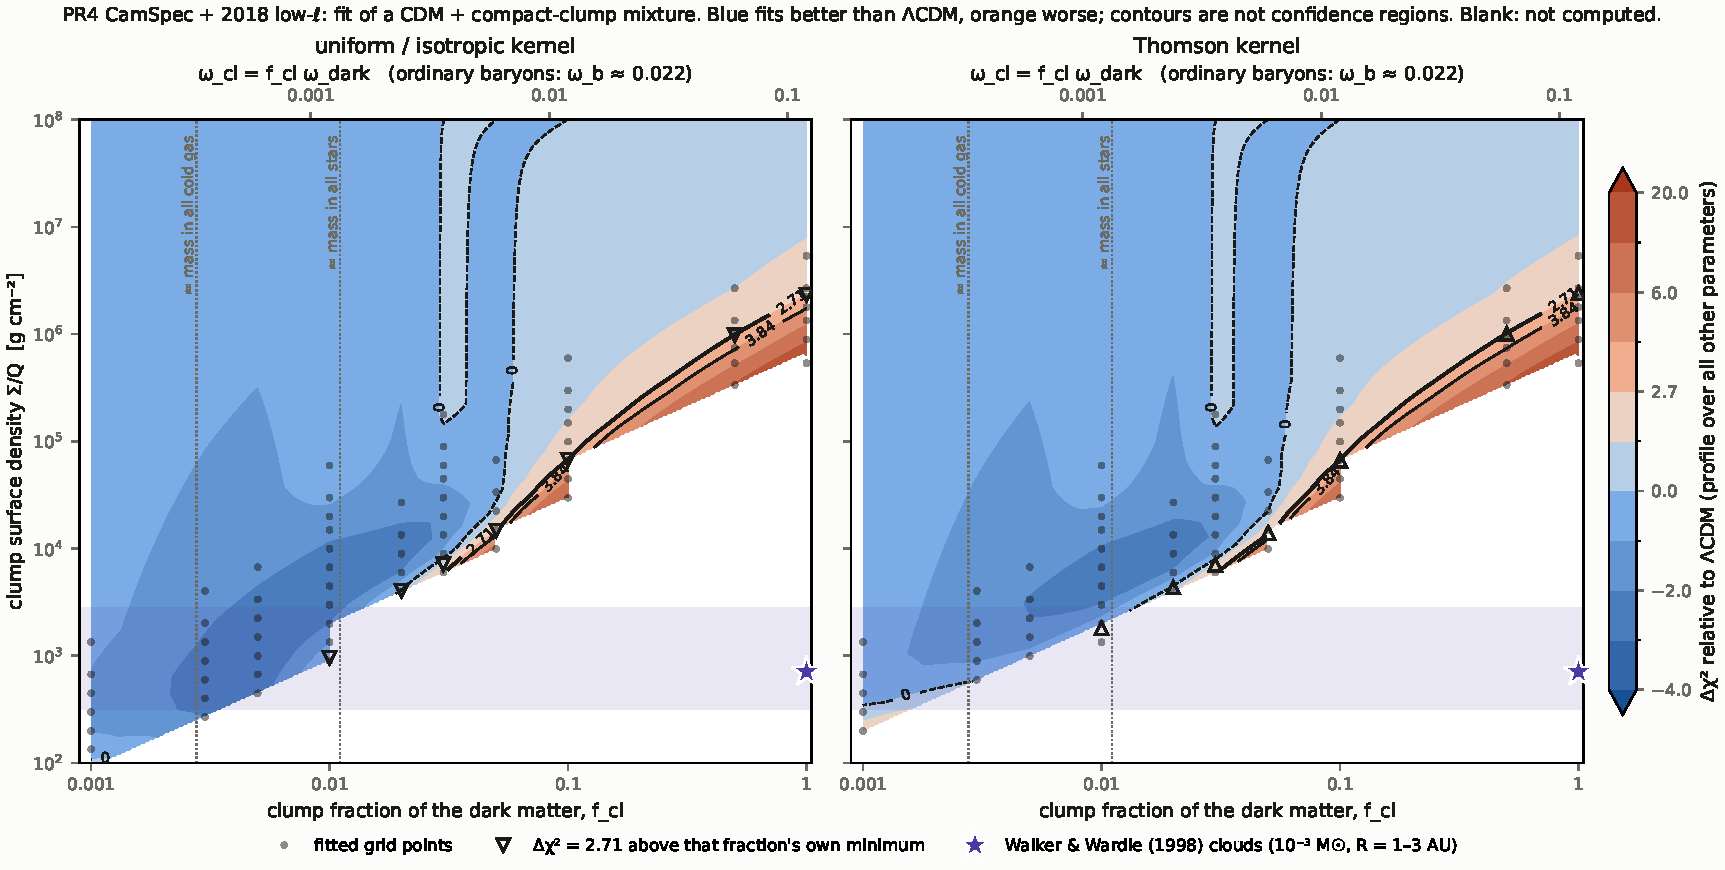
\includegraphics[width=\textwidth]{mix_contour_camspec_npipe.pdf}
\caption{$\dchi$ relative to $\Lambda$CDM as a function of clump fraction and surface density, for the isotropic (left) and Thomson (right) kernels. Blue regions fit as well as or slightly better than $\Lambda$CDM, orange regions worse. Triangles mark the fixed-fraction thresholds of Table~\ref{tab:thresholds}. The shaded band and star show the surface density of the clouds of \citet{WalkerWardle1998}. Dotted lines mark clump densities equal to the present-day mass in stars and in cold gas, as approximate fractions of the cosmic baryons. Blank regions were not computed.}
\label{fig:contour}
\end{figure}

Table~\ref{tab:thresholds} and Figure~\ref{fig:contour} summarise the results. Three points stand out.

\paragraph{CDM weakens the constraint, faster than $1/f_\cl$.} The drag suppresses only the clump perturbations, and after decoupling the CDM pulls the clumps back into its potential wells. The threshold on $u$ rises by a factor of 36 from $f_\cl = 1$ to $0.1$, and by about 1300 to $f_\cl = 0.01$. The minimum surface density falls correspondingly from $2\times10^{6}$ to about $10^{3}\,\mathrm{g\,cm^{-2}}$.

\paragraph{The kernel matters only at small fractions and strong coupling.} For $f_\cl \geq 0.02$ the two kernels give thresholds within about 7\%. For $f_\cl \lesssim 0.01$ the required coupling is large enough that the clumps carry an appreciable part of the photon scattering after recombination, and Thomson scattering off them generates polarization that the data disfavour. The isotropic kernel, which is the appropriate one for opaque clumps, allows lower surface densities there.

\paragraph{A shallow minimum below $\Lambda$CDM.} For $f_\cl \approx 0.003$--$0.02$ the profiles have a minimum at non-zero coupling, about 2.5 to 2.9 below $\Lambda$CDM in $\chi^2$. The improvement comes from the low-$\ell$ temperature spectrum and is accompanied by a higher spectral index ($n_s \approx 0.97$ instead of 0.961). It is the known deficit of Planck's low-$\ell$ temperature power, which other one-parameter extensions also fit. With two fitted parameters the significance is about $1.2\sigma$ ($p \approx 0.23$), lower once the search over the valley is accounted for. It is not evidence for clumps.

\subsection{Where the Walker \& Wardle clouds fall}

Clouds with $M \lesssim 10^{-3}\,M_\odot$ and radii of a few AU \citep{WalkerWardle1998} have $\Sigma \approx 3\times10^{2}$--$3\times10^{3}\,\mathrm{g\,cm^{-2}}$. On the CMB evidence alone:
\begin{itemize}
\item as all of the dark matter they are excluded by more than three orders of magnitude in $\Sigma$;
\item with the isotropic kernel they are allowed for $f_\cl \lesssim 0.01$, and lie in the region that fits as well as $\Lambda$CDM;
\item $f_\cl \approx 0.003$--$0.01$ corresponds to $\omega_\cl \approx (0.4$--$1.2)\times10^{-3}$, or 1.5--5\% of the cosmic baryons, comparable to the present-day mass in cold gas or in stars. In a Milky-Way halo of $10^{12}\,M_\odot$ it would be $(0.3$--$1)\times10^{10}\,M_\odot$ in clouds.
\end{itemize}

\section{Caveats}
\label{sec:caveats}

\paragraph{Existence through the acoustic epoch.} All of the above assumes the clumps exist, with the stated $\Sigma$, at redshifts of roughly $10^{3}$--$10^{5}$. For clouds like those of \citet{WalkerWardle1998} this assumption fails. A cloud of $10^{-3}\,M_\odot$ and radius 2\,AU has a virial temperature of order 100\,K. Held at the radiation temperature, it can be gravitationally bound only below $z \approx 50$ (the survival estimate in the explainer, Section~9). If such clouds form later, from gas that was diffuse at recombination, the CMB counts that gas as ordinary baryons and the drag constraint does not apply to them at all. The relevant constraint is then the baryon budget: the clouds must come out of the measured $\omega_b$, and so can be at most a fraction of the ordinary baryons, not a separate dark component.

\paragraph{Nucleosynthesis.} Clumps formed after BBN are counted as baryons by the light-element abundances, while the CMB counts them as dark matter. The agreement of the BBN and CMB baryon densities leaves room for an extra component of only a few per cent of $\omega_b$, which corresponds to $f_\cl \lesssim 0.01$. This figure depends on the nuclear reaction rates adopted and should be checked.

\paragraph{Scope of the model.} The limits hold only if the clumps are the sole departure from $\Lambda$CDM. A population of early compact objects would probably come with other changes, such as small-scale clumping of the remaining gas and a modified recombination history, that are not modelled and could move the limits in either direction.

\paragraph{Statistics.} The thresholds are fixed-fraction profile values. A Bayesian analysis with $f_\cl$ and $u$ both free is planned. At $f_\cl = 1$ it gave a limit 50\% weaker than the profile, so the boundary in Figure~\ref{fig:contour} may move by a similar factor.

\section{Points for discussion}

\begin{enumerate}
\item At what redshift do the clouds need to exist in the proposed scenario, and from what material do they form?
\item Is the intended cloud population within the baryon budget fixed by BBN and the CMB, or in addition to it?
\item Does the scattering-event model fix the cloud surface density independently? If so, the CMB constraint on $f_\cl$ at that fixed $\Sigma$ becomes a one-parameter test.
\item Which angular law is appropriate for photon interactions with the clouds at the relevant epochs: absorption and isotropic re-emission, or something closer to reflection?
\end{enumerate}

\begin{thebibliography}{9}
\bibitem[Walker \& Wardle(1998)]{WalkerWardle1998}
Walker M., Wardle M., 1998, \emph{Extreme scattering events and Galactic dark matter}, ApJ 498, L125.
\end{thebibliography}

\end{document}
